\documentclass{letter}

\usepackage[left=0.75in, right=0.75in, top=1.1in, bottom=0.75in]{geometry}
\usepackage{fancyhdr, amsmath, amssymb, mathtools, xcolor, graphicx, listings, mathpazo}
\graphicspath{{.}}

\pagestyle{fancy}
\fancyhf{}
\rhead{Page \thepage}
\chead{AMSC808N Homework 5}
\lhead{Tyler Hoffman}
\setlength{\headsep}{0.2in}

\newcounter{problem}
\newcounter{subproblem}[problem]
\newcounter{solution}

\renewcommand{\thesubproblem}{(\alph{subproblem})}

\newcommand{\Problem}[2]{%
	\stepcounter{problem}%
	\leftskip=0pt%
	\theproblem.~\textbf{{#1.}} #2 \par%
}

\newcommand{\Subproblem}[1]{%
	\stepcounter{subproblem}%
	\leftskip=15pt%
	\thesubproblem~ #1 \par%
}

\newcommand{\Solution}[1]{%
	\textbf{Solution.} #1 \par%
}

\newcommand{\Due}[1]{\textbf{Due: #1} \par}

\newcommand{\UNFINISHED}{\textbf{\color{red} UNFINISHED}}
\newcommand{\CHECK}{\textbf{\color{orange} CHECK ME}}

\newcommand{\iu}{{i\mkern1mu}}
\newcommand{\T}{\intercal}
\newcommand{\R}{\mathbb{R}}

\DeclareMathOperator{\diag}{diag}
\DeclareMathOperator{\rank}{rank}
\DeclareMathOperator{\nul}{nul}
\DeclareMathOperator{\tr}{tr}

\usepackage{hyperref}
\begin{document}
    \Due{19 Nov 2020}

    \Problem{Laplacian eigenmap}{Show that the Laplacian eigenmap to $\R^m$ is the solution to the following optimization problem: \begin{align*}
        \min\sum_{i, j} k_{ij}\|y_i - y_j\|_2^2 \hspace{5mm} \text{ subject to } \hspace{5mm} Y^\T Q Y = I, \hspace{5mm} Y^\T Q 1_{m\times 1} = 0.
    \end{align*} Here, the $y_i$ are rows of $Y \in \R^{n \times m}$ and the rest of the notation is as in the lecture notes. Also show that $\sum_{i, j} k_{ij}\|y_i - y_j\|^2_2 = \tr(Y^\T L Y)$ where $L$ is the graph Laplacian, $L = Q - K$.}
    \Solution{We begin by showing that $\sum_{i, j} k_{ij}\|y_i - y_j\|^2_2 = \tr(Y^\T L Y)$ using the fact that $K$ is symmetric and $q_i = \sum_j k_{ij}$. \begin{align*}
        \sum_{i, j} k_{ij}\|y_i - y_j\|^2_2 &= \sum_{i, j} k_{ij}(\|y_i\|^2 + \|y_j\|^2 - 2y_i^\T y_j) \\
        &= \sum_{i, j} k_{ij}\|y_i\|^2 + \sum_{i, j} k_{ij}\|y_j\|^2 - 2 \sum_{i, j} k_{ij}y_i^\T y_j \\
        &= \sum_i q_i \|y_i\|^2 + \sum_j q_j \|y_j\|^2 - 2 \sum_{i, j} k_{ij}y_i^\T y_j \\
        &= 2\tr(Y^\T Q Y) - 2\sum_{i, j} k_{ij}y_i^\T y_j.
    \end{align*} Next, we show that $\tr(Y^\T KY) = \sum_{i, j} k_{ij}y_i^\T y_j$. \begin{align*}
        \tr(Y^\T KY) &= \tr(KYY^\T) = \tr\left(K\begin{bmatrix} y_1 \\ \vdots \\ y_n\end{bmatrix}\begin{bmatrix} y_1^\T & \cdots & y_n^\T \end{bmatrix}\right) = \tr\left(K\begin{bmatrix} y_1y_1^\T & \cdots & y_1y_n^\T \\ \vdots & \ddots & \vdots \\ y_ny_1^\T & \cdots & y_ny_n^\T \end{bmatrix}\right) \\
        &= \tr\left(K\begin{bmatrix} y_1y_1^\T & \cdots & y_n^\T y_1 \\ \vdots & \ddots & \vdots \\ y_1^\T y_n & \cdots & y_n^\T y_n \end{bmatrix}\right) = \tr\left(\begin{bmatrix} \sum_i k_{1i} y_i^\T y_1 & \cdots & \sum_i k_{1i} y_i^\T y_n \\ \vdots & \ddots & \vdots \\ \sum_i k_{ni} y_i^\T y_1 & \cdots & \sum_i k_{ni} y_i^\T y_n \end{bmatrix}\right) \\
        &= \sum_j \sum_i k_{ji}y_i^\T y_j = \sum_{i, j} k_{ij} y_i^\T y_j
    \end{align*} which is exactly the same term as in the earlier calculation. So we see that \begin{align*}
        \sum_{i, j} k_{ij}\|y_i - y_j\|^2_2 = 2\tr(Y^\T QY) - 2\tr(Y^\T KY) = 2\tr(Y^\T LY)
    \end{align*} as desired (up to normalization by a factor of $1/2$). 
    
    We next have to prove that this trace is minimized by the Laplacian eigenmap to $\R^m$. Begin with the minimization problem $\min_Y \tr(Y^\T L Y)$ and impose the constraint $Y^\T Q Y = I$. This constraint removes a scale factor in the embedding---by forcing $Y^\T Q Y = I$, we're merely normalizing the embedded vectors $y_i$ under the inner product defined by $Q$. Next, we find the Lagrangian of this constrained optimization problem: \begin{align*}
        \mathbb{L} = \tr(Y^\T L Y) - \tr(\Lambda^\T (Y^\T QY - I))
    \end{align*} where $\Lambda$ is a diagonal matrix of Lagrange multipliers. Taking the derivative and setting it to zero gives \begin{align*}
        \frac{\partial \mathbb{L}}{\partial Y} = 2LY - 2QY\Lambda = 0 \implies LY = QY\Lambda
    \end{align*} which is exactly the generalized eigenvalue problem that we solve when we find the Laplacian eigenmap.
    
    To get the last constraint, we notice that an easy to see eigenpair is $(0, 1_{m\times 1})$: \begin{align*}
        L1_{m\times 1} = (Q - K)1_{m\times 1} = \begin{bmatrix} q_1 \\ \vdots \\ q_n \end{bmatrix} - \begin{bmatrix} \sum_j k_{1j} \\ \vdots \\ \sum_j k_{nj} \end{bmatrix} = 0.
    \end{align*} From this, we impose the constraint $Y^\T Q 1_{m\times 1} = 0$, meaning that all of the other eigenvectors must be orthogonal to $1_{m\times 1}$ under the inner product defined by $Q$. This allows us to eliminate the trivial eigenpair $(0, 1_{m\times 1})$ and makes it so the embedding works.}

    \Problem{Dimensional reduction comparison}{The goal of this problem is to practice and compare various methods for dimensional reduction. Use the following methods: \begin{itemize}
        \item PCA
        \item Isomap
        \item LLE
        \item t-SNE
        \item Diffusion maps.
    \end{itemize} Diffusion maps should be programmed from scratch, but the rest can be programmed using library functions. If you use library functions, specify their source, read their descriptions, and be ready to adjust their parameters. There are three datasets: \begin{itemize}
        \item an S-curve generated by a Matlab function
        \item an S-curve perturbed by Gaussian noise---try various intensities and push the methods' limits
        \item the ``emoji'' dataset generated by a Matlab function---picking a good $\epsilon$ for diffusion map might be tricky since the nearest neighbor distances are very nonuniform. You should be able to get a nice 2D surface in 3D with the right $\epsilon$. Use either $\alpha=0$ or $\alpha=1$ (up to you).
    \end{itemize} Submit a report on the performance of these methods on each dataset.}
    \Solution{My code can be found at \href{https://github.com/thoffman1/amsc808n}{this link}. I generated the datasets in Matlab and saved them to files, then read and processed them in Python. I used functions from the \texttt{scikit-learn} library to do PCA, Isomap, LLE, and t-SNE. Before I began, I compiled a brief list of the parameters I could change in these functions that would significantly affect the performance of the methods: \begin{itemize}
        \item PCA (none)
        \item Isomap \begin{itemize}
            \item \texttt{n\_neighbors} = number of neighbors to consider when constructing graph (default 5)
        \end{itemize}
        \item LLE \begin{itemize}
            \item \texttt{n\_neighbors} = number of neighbors to consider when constructing graph (default 5)
        \end{itemize}
        \item t-SNE \begin{itemize}
            \item \texttt{perplexity} = continuous measure of nearest neighbors (default 30, suggested $[5, 50]$)
            \item \texttt{early\_exaggeration} = controls how close together original clusters become in the embedded space (default 12)
            \item \texttt{learning\_rate} = step size for optimization problem. ``If the learning rate is too high, the data may look like a 'ball' with any point approximately equidistant from its nearest neighbours. If the learning rate is too low, most points may look compressed in a dense cloud with few outliers.'' (default 200, suggested $[10, 1000]$)
        \end{itemize}
        \item Diffusion map (custom code) \begin{itemize}
            \item \texttt{epsilon} = size of ball within which to look for neighbors. I followed Lafon and Lee (``Diffusion maps and coarse-graining: a unified framework for dimensionality reduction, graph partitioning, and data set parameterization''; 2006) and set $\epsilon = \frac{1}{n}\sum_{i=1}^n \min_{x_j \neq x_i} \|x_i - x_j\|^2$ so that it is adaptively adjusted based on the inputted data. However, there is still the option in my code to enter in a custom epsilon value.
            \item \texttt{delta} = accuracy of embedding; determines the power for the stochastic matrix (default 0.2)
            \item \texttt{alpha} = parameter for dealing with nonuniform data (default 0, suggested 0, $1/2$, or 1)
        \end{itemize}
    \end{itemize}
    
    \textbf{Dataset 1: Regular S-curve.} As noted in class, PCA did not unfold this dataset, but all the other methods provided decent embeddings into 3D. Isomap is perhaps the worst-performing here---the curves are jittery and not smooth as in all the other methods. Also as predicted, LLE provides a nice 2D manifold in $\R^3$. Since t-SNE is highly susceptible to initialization and parameters, I never got the same surface twice from it when I ran it, but they were all smooth and two-dimensional. Finally, diffusion map gives another smooth 2D manifold. Overall, all the methods worked satisfactorily on this dataset. See Figure 1 for plots.

    \textbf{Dataset 2: Noisy S-curves.} I processed a number of the noisy curves in Matlab, exported the data to .mat files, and read them into a Jupyter notebook for processing. See Figures 2-4 for the results of this processing. PCA continues to simply reproduce the noisy S-curve, which is all right but does not reflect much of the structure that underlies the data. In the least noisy S-curve (0.1, Figure 2), all the methods still work. However, most of them return dramatically different results than they did for the uniform S-curve---all except diffusion map, which remains a very similar shape. Continuing through 0.25 and 0.45 added noise (Figures 3 and 4, respectively), we see that similar patterns emerge: PCA still recreates the noisy curve, diffusion map reproduces the same manifold, and the other methods start to break down. LLE and Isomap crumble first, returning blurry blobs from any angle. t-SNE is hard to interpret at the 0.25 noise level and nearly unintelligible at the 0.45 noise level, but diffusion map stays strong. This is strong evidence that diffusion maps are highly robust to noise in a dataset and should be the method of preference of these five.

    \textbf{Dataset 3: Emojis.} Finally, in the emoji dataset, the trends continued. I did not remove the outlier emojis as keeping them in was a way to check that my methods were accurately working. Surprisingly (despite the data being highly nonlinear), PCA recovered the faces and the noise but did not represent the faces as varying in more than one dimension. Diffusion map had the best representation of the emojis, as it showed the faces and noise and captures the nonlinear curl in the data that the faces have. Isomap has the two outliers and weird spindly strands emerging from some odd origin, while t-SNE has extremely weird curls that are impossible to interpret. The worst performing method is LLE, which appears to simply not work on the data.

    In conclusion, diffusion map is by far the best method out of these five overall in terms of accuracy. PCA is probably the second best, as it is the fastest, nonparametric, and captures a good deal of the information in the data (including nonlinearities). However, it is not robust to noise and does not create the same surfaces that diffusion map does. The other three are generally poor methods on the datasets in question; even after trying many parameter combinations they still did not improve.

    \begin{center}
        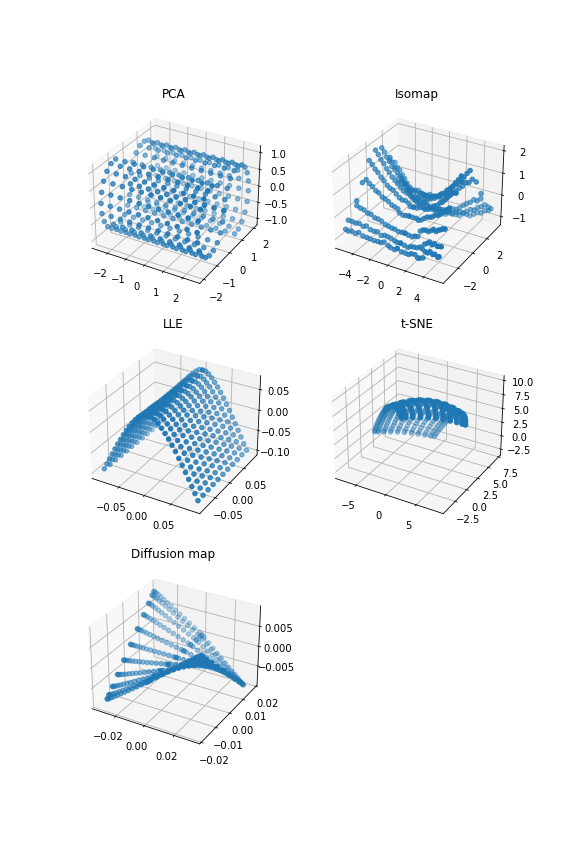
\includegraphics[scale=0.9, trim={2cm 2.5cm 1.5cm 3cm}, clip]{../pics/3d_scurve.png} \\
        Figure 1: Application of each method on the regular S-curve.
    \end{center}
    
    \begin{center}
        \includegraphics[scale=0.9, trim={2cm 2.5cm 1.5cm 3cm}, clip]{../pics/{noisy_scurve0.1}.png} \\
        Figure 2: Application of each method on the S-curve with $0.1$ added noise.
    \end{center}

    \begin{center}
        \includegraphics[scale=0.9, trim={2cm 2.5cm 1.5cm 3cm}, clip]{../pics/{noisy_scurve0.25}.png} \\
        Figure 3: Application of each method on the S-curve with $0.25$ added noise.
    \end{center}

    \begin{center}
        \includegraphics[scale=0.9, trim={2cm 2.5cm 1.5cm 3cm}, clip]{../pics/{noisy_scurve0.45}.png} \\
        Figure 4: Application of each method on the S-curve with $0.45$ added noise.
    \end{center}
    
    \begin{center}
        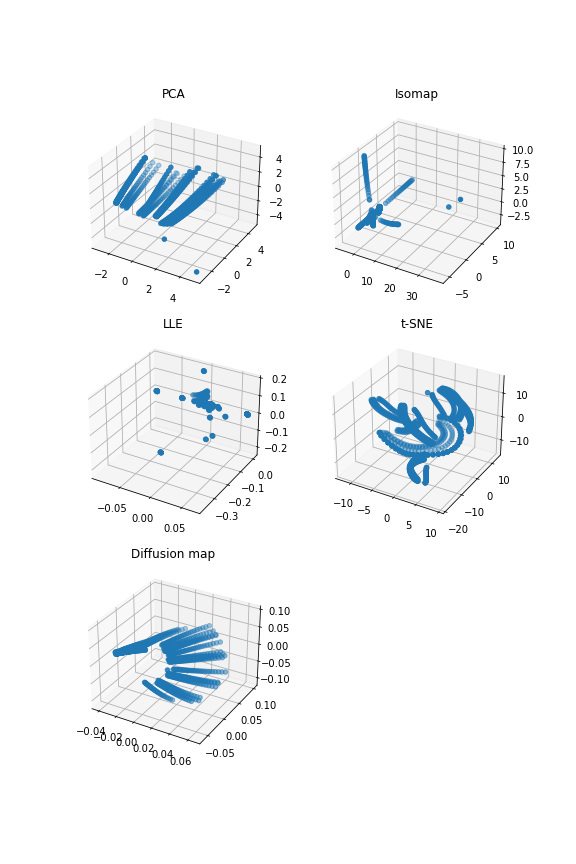
\includegraphics[scale=0.9, trim={2cm 2.5cm 1.5cm 3cm}, clip]{../pics/emoji.png} \\
        Figure 5: Application of each method on the emoji data.
    \end{center}}
\end{document}